\documentclass[class=article, crop=false, 12pt]{standalone}
\usepackage[subpreambles=true]{standalone}
\usepackage{../.common/common}

\author{Tony Shing}
%\pretitle{Supplementary}

\topic{Note 6B (Mechanics)}
\title{Angular Momentum and Rotational KE}

\version{2025} % leave blank for omitting

\begin{document}

\maketitle

%\heading{Lecture}{Tony}

\begin{overview}
    \begin{itemize}
        \item Formula review: Center of Mass \& Moment of Inertia of objects
        \item Mathematical Origin of 
        $\bcase{
            &\text{Angular Momemtum} \\ 
            &\text{Moment of Inertia} \\ 
            &\text{Parallel Axis Theorem}\\
            &\text{Rotational KE}
        }$
    \end{itemize}
\end{overview}



% content begins here
% Section %%%%%%%%%%%%%%%%%%%%%%%%%%%%%%%%%%%%%%%%%%%%%%%%%%%%
\section{Formula Review}

%%%%%%%%%%%%%%%%%%
\subsection{Center of Mass}
Given a set of point objects with individual masses $\{m_1, m_2, ..., m_n\}$ at positions $\{\vvec{r}_1, \vvec{r}_2, ..., \vvec{r}_n\}$,
the coordinate of center of mass of these objects can be calculate with the formula:
\aleq{
    \Aboxed{
        \vvec{r}_{CM} = \frac{m_1\vvec{r}_1 + m_2\vvec{r}_2 + ... + m_n\vvec{r}_n}{m_1+m_2+...+m_n} 
        = \frac{\sum_i^n m_i \vvec{r}_i}{\sum_i^n m_i}
    }
}

In case of a continuous distribution of masses, it becomes an integration:
\aleq{
    \Aboxed{
        \vvec{r}_{CM} 
        = \frac{\int \vvec{r}\dd{m}}{\int \dd{m}} 
        \sim \frac{\iiint \vvec{r}\rho \dd{x}\dd{y}\dd{z}}{M_\text{total}}
    }
}
with $\rho$ being the density as a function of position.

\vskip 1.5em
\underline{\textit{Proof}}\par
\hspace{0.025\textwidth}\begin{minipage}{0.95\linewidth}
\vskip 0.5em

    The formula can be proven by mathematical induction.\\

    \bf{\ul{Case $n=2$}}:\\
    Starting with 2 point masses $m_1$ and $m_2$. 
    the \bf{center of mass} is defined as \ul{the position} \ul{where if a normal force is applied, the whole object is in equilibrium}.\\

    \begin{center}
        \begin{minipage}{0.3\linewidth}
            \centering
            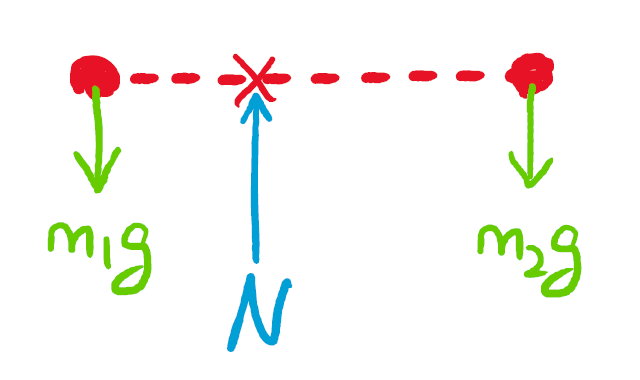
\includegraphics[width=0.8\textwidth]{cm_diag}\\
            Free body diagram
        \end{minipage}
        \hspace{0.15\textwidth}
        \begin{minipage}{0.3\linewidth}
            \centering
            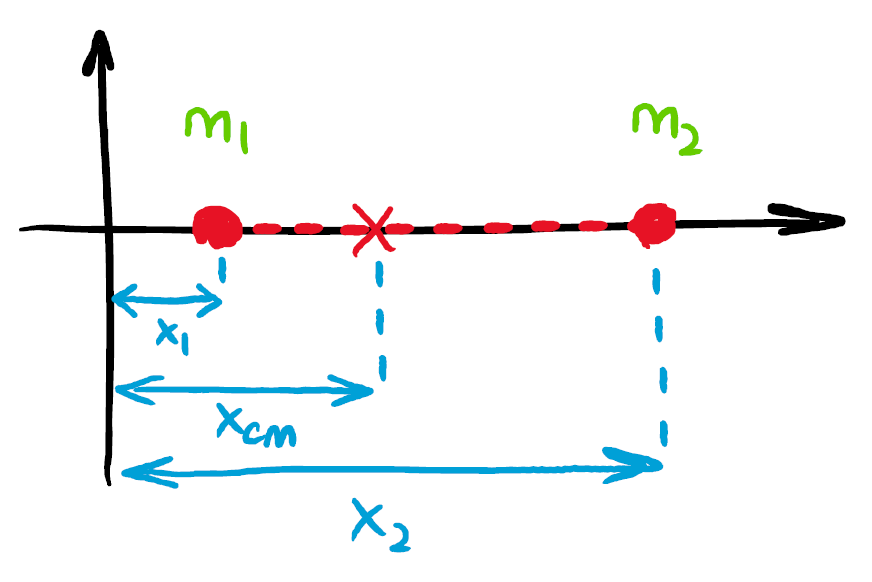
\includegraphics[width=\textwidth]{cm_pos}\\
            On coordinate system
        \end{minipage}
    \end{center}

\end{minipage}\\

\begin{minipage}{0.95\linewidth}
    We can assume both masses are on the x axis to simplify our visualization.
    Let the x coordinates of the masses be $x_1$ and $x_2$,
    and the coordinate of the center of mass be $x_\text{CM}$.
    If we choose the pivot at $x_\text{CM}$, 
    we only need to consider the torques and can ignore the normal force when writing Newton's \nth{2} law.
    \aleq{
        \anticlockwise :\quad  m_1g(x_\text{CM}-x_1) &= m_2g(x_2-x_\text{CM}) \\[1ex]
        (m_1+m_2)x_{CM} &= m_1x_1 + m_2x_2 \\[1ex]
        x_{CM} &= \frac{m_1x_1+m_2x_2}{m_1+m_2}
    }

    \bf{\ul{Case $n=k+1$}}:\\
    Assume the formula works for $k$ masses, i.e. 
    \aleq{
        x_\text{CM}^{(k)} = \frac{m_1x_1+m_2x_2 +...+ m_kx_k}{m_1+m_2+...+m_k} 
    }

    The center of mass is where the net torque under gravity = 0 by the two objects - 
    [Group of the first $k$ masses] and the [$(k+1)^\text{th}$ mass]
    \aleq{
        \anticlockwise :\quad  (m_1+m_2+...+m_k)g(x_\text{CM}^{(k+1)} - x_\text{CM}^{(k)}) &= m_{k+1}g(x_{k+1}-x_\text{CM}^{(k+1)}) \\[1ex]
        (m_1+m_2+...+m_k+m_{k+1})x_\text{CM}^{(k+1)} &= (m_1+m_2+...+m_k)x_\text{CM}^{(k)} + m_{k+1}x_{k+1} \\[1ex]
        &= (m_1x_1+m_2x_2+...+m_kx_k) + m_{k+1}x_{k+1} \\[1ex]
        x_\text{CM}^{(k+1)} &= \frac{m_1x_1+m_2x_2+...+m_{k+1}x_{k+1}}{m_1+m_2+...+m_{k+1}}
    }

    So the formula also works for $k+1$ masses.\\

    Because the same operation can be done on $y$ and $z$ coordinates, we can promote this formula to the vector expression
    \aleq{
        \vvec{r}_\text{CM} = \frac{m_1\vvec{r}_1+m_2\vvec{r}_2+...+m_n\vvec{r}_n}{m_1+m_2+...+m_n} 
    }

\hfill $\square$
\end{minipage}
\vskip 1.5em \par

%%%%%%
\subsection{Moment of Inertia}

It is common to ask for the moment of inertia of certain objects in solving rotation problems.
The \it{naive description} is that if a point mass $m$ is rotating around an axis with a radius $R$, 
then the mass is said to have a moment of inertia 
\aleq{
    I = mR^2 
}

If there are many masses,
then the "total" moment of inertia is just the sum of all of them.
\aleq{
    \Aboxed{
        I_\text{total} = m_1R_1^2 + m_2R_2^2 + \cdots m_nR_n^2 = \sum_i m_iR_i^2
    }
}

In case of a continuous distribution of masses, i.e. a rigid body,
it becomes an integration:
\aleq{
    \Aboxed{
        I_\text{total} 
        = \int \norm{\vvec{r}}^2\dd{m}
        \sim \iiint \norm{\vvec{r}}^2\rho \dd{x}\dd{y}\dd{z}
    }
}
with $\rho$ being the density as a function of position.\\

Multiple integral is the essential tool to compute moment of inertia of objects.

\begin{example}
    Consider a hemisphere of radius $R$ with a density $\rho(r,\theta,\phi) = 1+r^2$ as a function of radius only.
    The moment of inertia about the central axis is a straightforward multiple integral using spherical coordinate. 
    
    \begin{center}
        \begin{minipage}{0.2\linewidth}
            \centering
            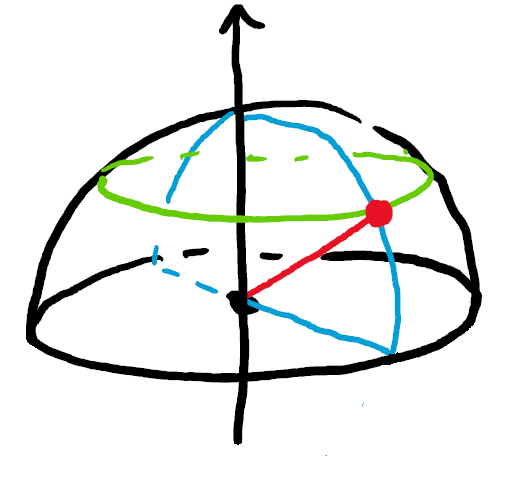
\includegraphics[width=\textwidth]{hemisphere}
        \end{minipage}
    \end{center}

    \aleq{
        I &= \iiint r^2 \dd{m} \\[1em]
        &= \int_0^R \int_{0}^{\frac{\pi}{2}} \int_0^{2\pi} r^2 \cdot \rho\cdot r^2\sin\theta\dd{\phi}\dd{\theta}\dd{r} \\[1em]
        &= \int_0^R \int_{0}^{\frac{\pi}{2}} \int_0^{2\pi} r^2(1+r^2) \cdot r^2 \sin\theta\dd{\phi}\dd{\theta}\dd{r} \\[1em]
        &= \int_0^R r^2(1+r^2) \cdot \tkn{hemi}{\cul[blue]{2\pi r^2 \dd{r}}} \\[1em]
        &= 2\pi\qty(\frac{R^5}{5} + \frac{R^7}{7})
    }
    \addBentArrow[blue]{hemi}{(10ex,-3ex)}{\scriptsize Area of half a sphere shell = $2\pi r^2$ \\[-1ex]\scriptsize thickness = $\dd{r}$}
    {(0,-1ex)}{(10ex,1ex)}

\end{example}


\linesep
\newpage
%%%%%%%%%%%%%%%%%%%%%%%%%%%%%%%%%%%%%%%%%%%%%%%%%%%%%%%%%%%%%%%%%%%%%%%%%%%%%%%%%%%
\section{Torque, Angular Momentum \& Moment of Inertia}

%%%%%%
\subsection{Origin of Idea}

Recall that if $\dd{\vvec{r}}/\vvec{v}/\vvec{a}$ are given, 
we can isolate their angular components $\dd{\theta}/\omega/\alpha$ by taking $\vvec{r}\cross$. 
We can do the same to force $\vvec{F}$
to arrive at the definition of \bf{torque}.
\aleq{
    \Aboxed{\vvec{\tau} &\defeq \vvec{r}\cross \vvec{F}}
}

Continue deriving,
\aleq{
    \vvec{\tau} &\defeq \vvec{r}\cross \vvec{F} \\[1ex]
    &= r\hhat{r} \cross m\vvec{a} \\[1ex]
    &= rma_\theta \hhat{z} \\[1ex]
    &= rm\qty[2\dvv{r}{t}\cdot\dvv{\theta}{t} 
        + r\cdot \dvv[2]{\theta}{t}]\hhat{z} &(\text{\scriptsize Just the Corriolis and Euler terms})\\[1ex]
    &= m\qty[\dvv{r^2}{t}\cdot\dvv{\theta}{t} 
        + r^2\cdot \dvv[2]{\theta}{t}]\hhat{z} &({\scriptstyle \text{ \nth{1} term: }2r\dd{r} \ \to\  \dd{(r^2)} })\\[1ex]
    &= \dvv{t}\qty(mr^2\dv{\theta}{t})\hhat{z} &(\text{\scriptsize product rule})\\[1ex]
    &= \dvv{t}\qty(\vvec{r}\cross (m\vvec{v}))
}

Comparing with relations between force and momentum, we can define a similar quantity that represents the angular component of momentum,
i.e. the \bf{angular momentum} $L$,
\aleq{
    \vvec{F} = \dvv{t}(m\vvec{v}) = \dvv{t}\qty(\text{momentum}) 
    \qquad\text{v.s.}\qquad 
    \vvec{\tau} = \dvv{t}\qty(mr^2\dvv{\theta}{t}\hhat{z}) 
        = \dvv{t}\qty(\mstack{\text{Something}\\\text{momentum-like}})
}
\aleq{
    \Aboxed{\vvec{L} \defeq \vvec{r}\cross (m\vvec{v}) = mr^2\dvv{\theta}{t}\hhat{z}}
}

\vskip 1em
And since momentum is the product of an inertia quantity (mass) and velocity, 
we can propose that the angular momentum is also a product of some new inertial quantity and the velocity in rotation (angular velocity).
So we arrive at the definition of \bf{moment of inertia} $I$.
\aleq{
    \vvec{p}=m\vvec{v} = (\text{inertia})\cdot(\text{velocity}) 
    \qquad\text{v.s.}\qquad 
    \vvec{L} = (mr^2)\cdot \dv{\theta}{t} 
        = \qty(\mstack{\text{something}\\\text{related to}\\[0.4ex]\text{inertia}})\cdot \qty(\mstack{\text{Angular}\\\text{velocity}})
}
\aleq{
    \Aboxed{I \defeq mr^2}
}

\vskip 1em
%%%%%%%%%%%%%%
\subsection{Rules of Using Rotational Quantities}

Unlike their linear motion counterparts, 
the rotational motion quantities are not universal.

\begin{enumerate}
    \item \bf{\ul{Angular quantites dependent on the choice of coordinate system}}

    \begin{center}
        \begin{minipage}{0.5\linewidth}
            \centering
            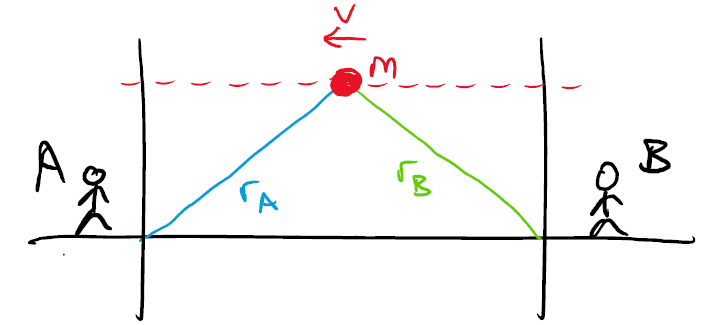
\includegraphics[width=\textwidth]{coor_depend}
        \end{minipage}
    \end{center}

    As illustrated, observers from different coordinate system describe 
    the same object with different position vectors,
    so their observed angular velocity, torque, angular momentum, and moment of inertia are all different. 
    \begin{table}[h!]
    \centering
        \begin{tabular}{ccc}
        & Observed by A & Observed by B \\ 
        \hline \hline
        $\vvec{\omega}$ & $\vvec{r}_A\cross\vvec{v}$ & $\vvec{r}_B\cross\vvec{v}$ \\ 
        \hline
        $\vvec{\tau}$ & $\vvec{r}_A\cross\vvec{F}$ & $\vvec{r}_B\cross\vvec{F}$ \\ 
        \hline
        $\vvec{L}$ & $\vvec{r}_A\cross(m\vvec{v})$ & $\vvec{r}_B(m\cross\vvec{v})$ \\ 
        \hline
        $I$ & $m \norm{\vvec{r}_A}^2$ & $m\norm{\vvec{r}_B}^2$ 
        \end{tabular}
    \end{table}

    In other words, \red{you should always fix the origin when writing formulas}.
    (From experience, you almost never see problems that require you to change origin.)
    %

    \item \bf{\ul{$I$ is not always well-defined in multi-body system}}

    Suppose we have many objects moving with their individual velocities.
    As we know that the net torque can be found by summing each object's contribution,
    so does the angular momentum. 

    \begin{center}
        \begin{minipage}{0.4\linewidth}
            \aleq{
                \vvec{\tau}_\text{total} &= \sum_i \vvec{\tau}_i  \\
                \quad\Rightarrow\quad 
                \vvec{L}_\text{total} &= \int \vvec{\tau}_\text{total} \dd{t} \\
                &= \sum_i \qty(m_i \vvec{r}_i\cross\vvec{v}_i) 
                = \sum_i \qty(m_i \norm{\vvec{r}_i}^2\vvec{\omega}_i)
            }
        \end{minipage}
        \hspace{0.05\textwidth}
        \begin{minipage}{0.25\linewidth}
            \centering
            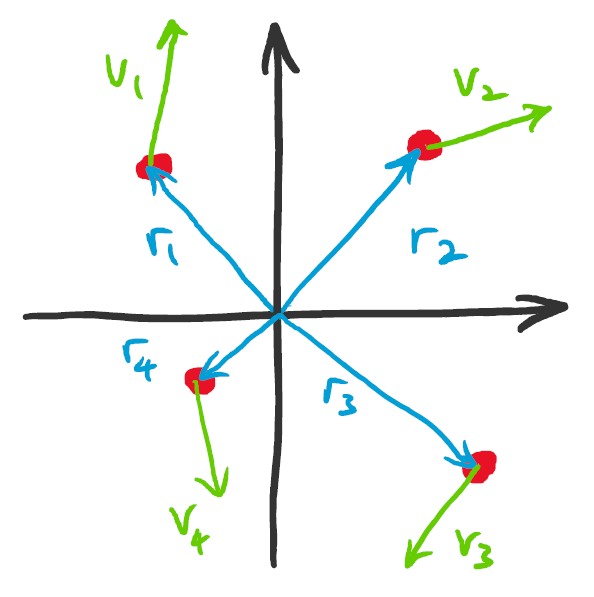
\includegraphics[width=\textwidth]{many_body_I}
        \end{minipage}
    \end{center}
    
    But in general cases, there is no way to take out $m\norm{\vvec{r}}^2$ from the summation, 
    and thus the moment of inertia is not well-defined. 
    Except when all objects move with the same $\omega$ about the same center,
    e.g. \red{the case of rigid body,
    only then we can define a total moment of inertia}.
    \aleq{
        \vvec{L}_\text{total} = \sum_i \qty(m_i \norm{\vvec{r}_i}^2\blue{\vvec{\omega}}) 
        = \qty(\sum_i m_i\norm{\vvec{r}_i}^2)\blue{\vvec{\omega}} = I_\text{total}\ \blue{\vvec{\omega}}
    }
    
\end{enumerate}

\begin{example}
    Compute the angular momentum as a function of time for an object moving in a circular trajectory,
    which is centered at $(x_0,y_0)$ with radius $R$.
    Let the object's mass be $m$ and moving at constant velocity $v$, 
    and is at the north of the circle at $t=0$.
    
    \begin{center}
        \begin{minipage}{0.4\linewidth}
            \centering
            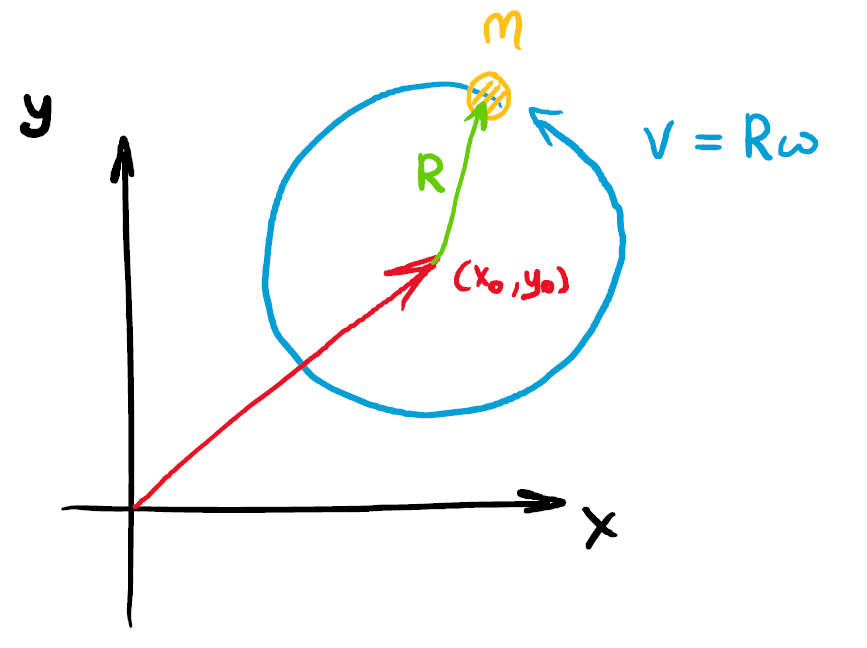
\includegraphics[width=\textwidth]{circ_track}
        \end{minipage}
    \end{center}

    By parametrizing the trajectory, we have the position vector of the mass as
    \aleq{
        \vvec{r}(t) = (x(t), y(t)) \quad\text{with}\quad
        \bcase{
            x(t) &= x_0 + R\cos{\qty(\frac{v}{R}t +\frac{\pi}{2})}\\
            y(t) &= y_0 + R\sin{\qty(\frac{v}{R}t +\frac{\pi}{2})}\\
        }
    }
    
    Differentiation gives its velocity vector:
    \aleq{
        \vvec{v}(t) = (v_x(t), v_y(t)) \quad\text{with}\quad
        \bcase{
            v_x(t) &= -v\sin{\qty(\frac{v}{R}t +\frac{\pi}{2})}\\
            v_y(t) &= v\cos{\qty(\frac{v}{R}t +\frac{\pi}{2})}\\
        }
    }

    Its angular momentum is then
    \aleq{
        \norm{\vvec{L}} &= \norm{m\vvec{r}\cross\vvec{v}} \\
        &= m(x(t)v_y(t) - y(t)v_x(t)) \\
        &= m\left[\qty(x_0 + R\cos{\qty(\frac{v}{R}t +\frac{\pi}{2})})\qty(v\cos{\qty(\frac{v}{R}t +\frac{\pi}{2})})\right.\\
        &\qquad\qquad - \left.\qty(y_0 + R\sin{\qty(\frac{v}{R}t +\frac{\pi}{2})})\qty(-v\sin{\qty(\frac{v}{R}t +\frac{\pi}{2})})\right]\\
        &= mx_0v\cos{\qty(\frac{v}{R}t +\frac{\pi}{2})} + my_0v\sin{\qty(\frac{v}{R}t +\frac{\pi}{2})} + mRv
    }

    which contains addition terms other than the usual form $L=mRv$. 
    Moreover, it is a function of $t$, so it is NOT conserved.
    We get this result because:
    \begin{itemize}
        \item The object is in a circular motion. 
        Linear momentum $mv$ cannot be conserved at all.

        \item Angular momentum is just the angular component of linear momentum.
    \end{itemize}

    Please beware of that in circular motion,
    $L=mRv$ is a conserved quantity only if the origin is chosen to be the center of the circular trajectory.
    
\end{example}

\newpage
%%%%%%%%%%%%%%%%%%%%%%%%%%%%%%
\subsection{Motions Relative to Center of Mass}

In many scenerios, 
rotation of objects are not about a fixed center. E.g. 
\begin{itemize}
    \item Satallite system: The Moon is rotating around the Earth, 
    which the Earth is rotating around the sun.
    \item Rolling: The masses are rotating about the cylinder/sphere's center, 
    which its center is moving in a straight line along the floor.
\end{itemize}

Remember, \red{the first rule of analyzing rotation motions is that you must use a fixed origin}. 
So in the above examples, you should still choose the sun / the floor as the origin.

\begin{center}
    \begin{minipage}{0.45\linewidth}
        \centering
        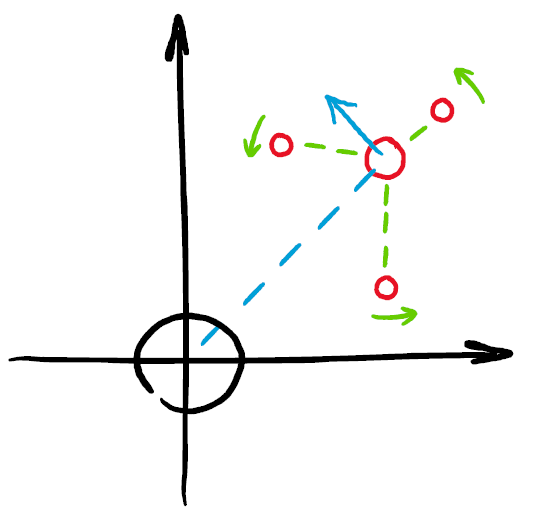
\includegraphics[height=10em]{satallite}\\
        The sun is a fixed point\\and is also a rotation center. 
    \end{minipage}
    \hspace{1.5em}
    \vline
    \hspace{1.5em}
    \begin{minipage}{0.45\linewidth}
        \centering
        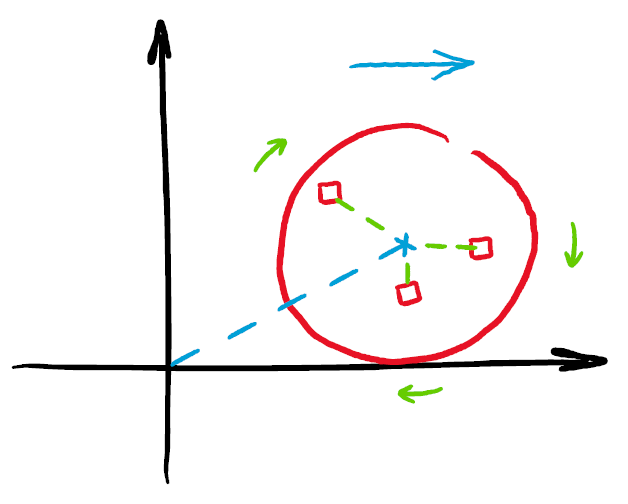
\includegraphics[height=10em]{rolling}\\
        Any points on the floor is a fixed point,\\
        although they are not rotation centers.
    \end{minipage}
\end{center}

%\vskip 2em
However this causes a lot of complications because the position vector $\vvec{r}$ and velocity vector $\vvec{v}$ 
to each point are not perpendicular. 
Calculating the total torque or angular momentum requires integration over cross products.
\aleq{
    \vvec{\tau} = \sum_{i} \vvec{r}_i\cross\vvec{F}_i \ &\to\  \int \vvec{r}\cross\dd{\vvec{F}} \\
    %
    \vvec{L} = \sum_{i}m_i\vvec{r}_i\cross \vvec{v}_i = \sum_{i} m_i\norm{\vvec{r}_i}^2\omega_i 
        \ &\to \ \int \vvec{r}\cross \vvec{v}\dd{m} = \int \norm{\vvec{r}}^2\omega \dd{m}
}


A proper treatment is to separate the position vectors (and velocity vectors) of the objects into two parts - 
the position vector of the center of mass $\vvec{r}_{CM}$, 
and the displacement vectors of each object relative to the center of mass $\vvec{R}_{i}$.
\aleq{
    \bcase{
        \vvec{r}_i &= \vvec{r}_{CM} + \vvec{R}_{i} \\
        \vvec{v}_i &= \vvec{v}_{CM} + \vvec{V}_{i} 
            \quad\qty(= \dvv{\vvec{r}_i}{t} = \dvv{\vvec{r}_{CM}}{t} + \dvv{\vvec{R}_i}{t} )
    }
}

%\vskip 1em
\begin{center}
    \begin{minipage}{0.95\linewidth}
        \centering
        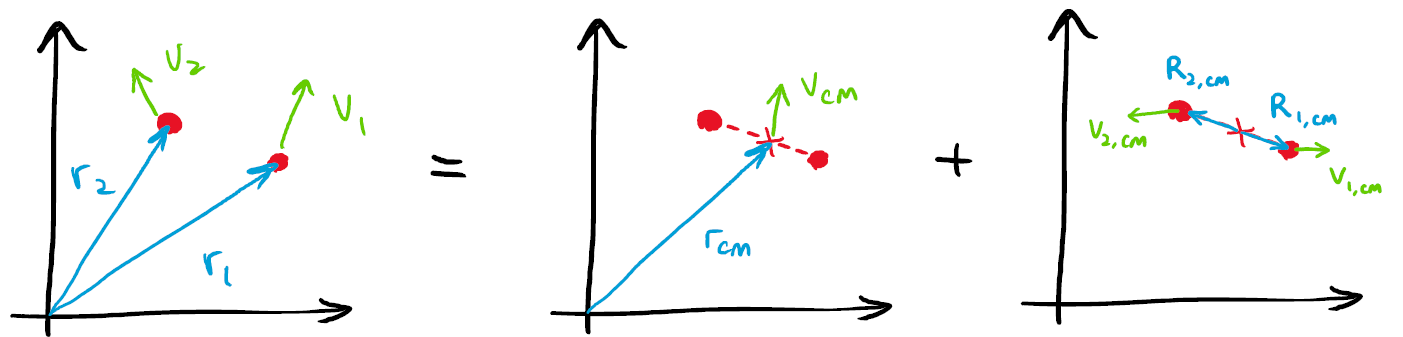
\includegraphics[width=\textwidth]{r_cm}
    \end{minipage}
\end{center}

\vskip 1em
Substitute them into the definition of angular momentum, we get
\addArrow[red]{L1}{(0,-2ex)}{\scriptsize Moment of inertia of\\[-1ex]\scriptsize a point mass $M_\text{total}$\\[-1ex]\scriptsize relative to origin}
{(0, -1.5ex)}{(0, -2ex)}
\addArrow[blue]{L2}{(0,-2ex)}{\scriptsize Moment of inertia of\\[-1ex]\scriptsize each object relative to CM}
{(0, -2.2ex)}{(0, -1.4ex)}
\addArrow[red]{L3}{(0,3ex)}{}{(0,2.5ex)}
\addArrow[blue]{L4}{(6ex,4ex)}{}{(0,2.5ex)}
\aleq{
    \vvec{L} &= \sum_i (m_i \vvec{r}_i\cross \vvec{v}_i) \\
    %
    &= \sum_i\qty[m_i(\vvec{r}_\text{CM}+\vvec{R}_i)\cross(\vvec{v}_\text{CM}+\vvec{V}_i)] \\
    %
    &= \sum_i m_i\qty[\vvec{r}_\text{CM}\cross\vvec{v}_\text{CM} + \vvec{r}_\text{CM}\cross\vvec{V}_i + \vvec{R}_i\cross\vvec{v}_\text{CM} + \vvec{R}_i\cross\vvec{V}_i] \\
    %
    &= \qty(\sum_i m_i)\qty[\vvec{r}_\text{CM}\cross\vvec{v}_\text{CM}] 
        + \vvec{r}_\text{CM}\cross\cus[green]{\ccancelto[green]{0}{\qty[\sum_i m_i\vvec{V}_i]}}{\substack{\text{Total velocity}\\\text{relative to CM = 0}}}
        + \cus[green]{\ccancelto[green]{0}{\qty[\sum_i m_i\vvec{R}_i]}}{\substack{\text{Total displacement}\\\text{from CM = 0}}}
            \cross\vvec{v}_\text{CM} 
        + \sum_i \qty[m_i \vvec{R}_i \cross\vvec{V}_i] \\
    %
    &= \cus[red]{\red{\qty(\sum_i m_i)\qty[\vvec{r}_\text{CM}\cross\vvec{v}_\text{CM}]}}{\substack{\text{Angular momentum of}\\\text{CM's motion about origin}}}
        \quad +\ \cus[blue]{\blue{\sum_i \qty[m_i \vvec{R}_i \cross\vvec{V}_i]}}{\substack{\text{Angular momentum of}\\\text{all object's motion about CM}}}\\[1em]
    %
    &= \quad\tkn{L1}{\cul[red]{\qty(M_\text{total}\norm{\vvec{r}_\text{CM}}^2)}}\vvec{\omega}_\text{CM}
    \quad+\quad 
    \sum_i \qty[\tkn{L2}{\cul[blue]{m_i\norm{\vvec{R}_i}^2}}\vvec{\Omega}_i] \\[3em]
    %
    &= \quad \tkn{L3}{\cul[red]{M_\text{total}\norm{\vvec{r}_\text{CM}}^2}}\vvec{\omega}_\text{CM} 
    \quad+\quad 
    \sum_i \qty[\tkn{L4}{\cul[blue]{I_{i,\text{CM}}}}\ \vvec{\Omega}_i]
} 




So we can write a system's angular momentum by combining the \cul[red]{center of mass's motion} 
and \cul[red]{objects's motion around the center of mass},
which simplifies the calculation in many problems.\\

\begin{notation}[]
    \begin{center}
        \red{\bf{\ul{We can only use the center of mass for such breakdown.}}}
    \end{center}
    $\sum_i\qty(m_i\vvec{R}_i)$ and $\sum_i\qty(m_i\vvec{V}_i) = 0 $ is true only if we take CM as the reference point. 
    We can prove $\sum_i\qty(m_i\vvec{R}_i) = 0$ using the CM formula.
    Then differentiate to get $\sum_i\qty(m_i\vvec{V}_i) = 0$.
    \aleq{
        \sum_i\qty(m_i\vvec{R}_i) &= \sum_i\qty[m_i(\vvec{r}_i - \vvec{r}_\text{CM})] \\
        &= \sum_i\qty(m_i\vvec{r}_i) - \qty(\sum_i m_i)\vvec{r}_\text{CM} \\
        &= \sum_i\qty(m_i\vvec{r}_i) - \cancel{\qty(\sum_i m_i)}\qty(\frac{\sum_i m_i\vvec{r}_i}{\cancel{\sum_i m_i}})\\
        &= 0
    }
\end{notation}

\begin{example}
    (Satellite motion)\\

    The Mars has two satellites Phobos and Deimos. The Mars is also revolving around the sun.
    Given the following data:
    \begin{itemize}
        \item Mass of Sun, Mars, Phobos and Deimos are $m_S$, $m_M$, $m_P$, $m_D$. Assume $m_S\gg m_M\gg m_P\approx m_D$
        \item Assume all orbits are circle. 
            Distance between Mars \& Sun = $r_{MS}$, between Mars \& Phobos = $r_{PM}$, between Mars \& Deimos = $r_{DM}$.
        \item Mars, Phobos and Deimos are self-rotating with angular velocity $\omega_M$, $\omega_P$, $\omega_D$.
        \item Moment of inertia of Mars, Phobos and Deimos about their center are $I_M$, $I_P$, $I_P$.
        \item Assume the Sun does not move or rotate at all.
    \end{itemize}
    
    \begin{center}
    \begin{minipage}{0.25\linewidth}
        \centering
        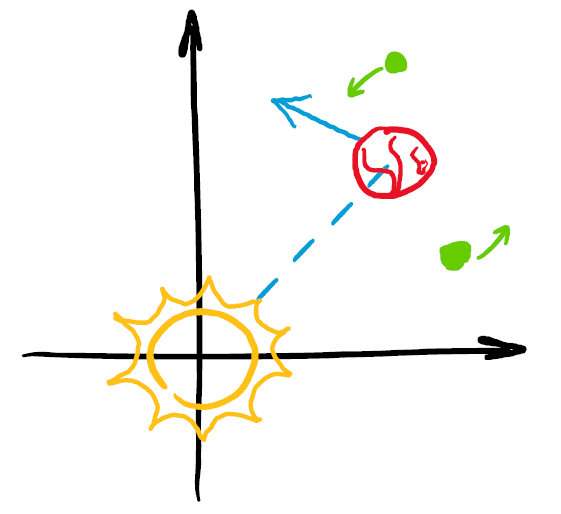
\includegraphics[width=\textwidth]{mars}
    \end{minipage}
\end{center}

    By gravity, the traveling speed of objects in circular motion is
    \aleq{
        \frac{GMm}{r^2} = \frac{mv^2}{r} \qquad\Rightarrow\qquad v=\sqrt{\frac{GM}{r}}
    }

    So the revolving speed for Mars, Phobos and Deimos are 
    \aleq{
        v_M = \sqrt{\frac{GM_S}{r_M}} \quad,\quad v_P = \sqrt{\frac{GM_M}{r_P}} \quad,\quad v_D = \sqrt{\frac{GM_M}{r_D}}
    }

    Taking the sun's center as the origin. 
    Because $m_M\gg m_P\approx m_D$, 
    the system's center of mass can be assumed at the Mars's center.
    We can write down the total angular momentum as
    \aleq{
        L &= M_\text{total}r_\text{CM}v_\text{CM} + \sum_i L_{i,\text{CM}} \\
        %
        &= \tkn{mars1}{\cul[red]{(m_M+m_P+m_D)r_{MS}v_M}} 
            + \tkn{mars2}{\cul[blue]{L_{(\text{Mars,CM})} + L_{(\text{Phobos,CM})} + L_{(\text{Deimos, CM})}}}\\[3.5em]
        %
        &= (m_M+m_P+m_D)r_{MS}v_M + \tkn{mars3}{\cub[blue]{I_M\omega_M}{\substack{\text{Mars' body}\\\text{is in}\\\text{rigid body}\\\text{rotation}}}}
            + \tkn{mars4}{\cub[green]{m_Pr_{PM}v_P + \sum_i L_{(i,\text{Phobos})}}
            {\substack{\text{Angular momentum of Phobos'}\\\text{center rotating around Mars}\\\text{+ anything rotating about}\\\text{Phobos' center}}}}
            + \tkn{mars5}{\cub[yellow]{m_Dr_{DM}v_D + \sum_i L_{(i,\text{Deimos})}}
            {\substack{\text{Angular momentum of Deimos'}\\\text{center rotating around Mars}\\\text{+ anything rotating about}\\\text{Deimos' center}}}}\\[0.5em]
        %
        &= (m_M+m_P+m_D)r_{MS}v_M + I_M\omega_M + m_Pr_{PM}v_P + \tkn{mars6}{\cul[green]{I_P\omega_P}} + m_Dr_{DM}v_D + \tkn{mars7}{\cul[yellow]{I_D\omega_D}}
    }
    \addArrow[red]{mars1}{(0,-2ex)}{\scriptsize Angular momentum of a point mass\\[-1ex]\scriptsize of mass $(m_M+m_P+m_D)$}
    {(0,-1.5ex)}{(0,-1.5ex)}
    \addArrow[blue]{mars2}{(0,-2ex)}{\scriptsize Angular momentum of\\[-1ex]\scriptsize anything rotating around Mars' center\\[-1ex]\scriptsize = Mars's body + Phobos + Deimos}
    {(0,-1.5ex)}{(0,-2ex)}
    \addArrow[blue]{mars3}{(8ex,4ex)}{}{(0,1.5ex)}
    \addArrow[green]{mars4}{(-1ex,4ex)}{}{(-2ex,1.5ex)}
    \addArrow[yellow]{mars5}{(-30ex,4ex)}{}{(-2ex,1.5ex)}
    \addArrow[green]{mars6}{(0,-2ex)}{\scriptsize Things rotating around Phobos\\[-1ex]\scriptsize = its own body mass\\[-1ex]\scriptsize in rigid body rotation}
    {(0,-1ex)}{(-3ex,-2ex)}
    \addArrow[yellow]{mars7}{(0,-2ex)}{\scriptsize Things rotating around Deimos\\[-1ex]\scriptsize = its own body mass\\[-1ex]\scriptsize in rigid body rotation}
    {(0,-1ex)}{(3ex,-2ex)}
    

\end{example}






%%%%%%%%%%%%%%%%%%%%%%%%%%%%%
\subsection{Parallel Axis Theorem}

The second rule of using angular quantities is that moment of inertia is well-defined
only when all masses rotate at the same angular velocity about the same center.
In such cases, we can always choose the rotation center as the origin. 

\begin{center}
    \begin{minipage}{0.4\linewidth}
        \centering
        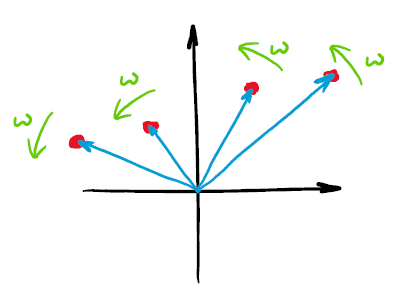
\includegraphics[height=10em]{same_omega}\\
        Applicable only if all objects moving\\
        at the same angular velocity $\omega$\\
        \cul[red]{relative to the origin}.
    \end{minipage}
    \hspace{2em}
    \vline
    \hspace{2em}
    \begin{minipage}{0.4\linewidth}
        \centering
        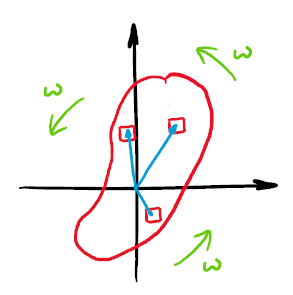
\includegraphics[height=10em]{rigid_body}\\
        Rigid body is equivalent to\\
        many small mass $\dd{m}$ rotating\\
        at the same angular velocity $\omega$.
    \end{minipage}
\end{center}

The angular momentum writes as:
\aleq{
    \vvec{L} &= \sum_i (m_i \vvec{r}_i\cross \vvec{v}_i) \\
    %
    &= \sum_i(m_i\norm{\vvec{r}_i}^2)\tkn{omegaO}{\cul[red]{\vvec{\omega}_O}} \\
    %
    &= \sum_i(m_i\norm{\vvec{r}_\text{CM}+\vvec{R}_i}^2)\vvec{\omega}_O \\
    %
    &= \qty[\sum_i \qty(m_i \norm{\vvec{r}_\text{CM}}^2) 
        + \sum_i\qty(m_i \norm{\vvec{R}_i}^2) 
        + 2\tkn{omegaCM}{\cul[green]{\ccancelto[green]{0}{\sum_i\qty(m_i \vvec{r}_\text{CM}\cdot\vvec{R}_i)}}}]\vvec{\omega}_O \\
    %
    &= \qty[\tkn{ICMO}{\cul[red]{M_\text{total}\norm{\vvec{r}_\text{CM}}^2}}
         + \tkn{ICM}{\cul[blue]{\sum_i\qty(m_i \norm{\vvec{R}_i}^2)}}]\vvec{\omega}_O\\[3.2em]
    %
    &= \qty[\tkn{ICMO2}{\cul[red]{I_{\text{CM},O}}} + \tkn{ICM2}{\cul[blue]{I_{i,\text{CM}}}}]\vvec{\omega}_O
}
\addArrow[red]{omegaO}{(5ex,0)}{\scriptsize All objects have\\[-1ex]\scriptsize the same angular velocity\\[-1ex]\scriptsize relative to $O$}
{(2.5ex,0)}{(9ex,0)}
\addArrow[green]{omegaCM}{(0,-3ex)}{$=\,\vvec{r}_{CM}\cdot\qty(\sum_i m_i\vvec{R}_i) =\, \vvec{r}_{CM}\cdot 0$}
{(0,-4ex)}{(10ex,-0.5ex)}
\addArrow[red]{ICMO}{(0,-3ex)}{\scriptsize Moment of inertia of\\[-1ex]\scriptsize a point with mass $M_\text{total}$\\[-1ex]\scriptsize relative to origin}
{(0,-1.5ex)}{(-2ex,-2ex)}
\addArrow[blue]{ICM}{(0,-3ex)}{\scriptsize Moment of inertia\\[-1ex]\scriptsize relative to CM}
{(0,-3.6ex)}{(0,-1ex)}
\addArrow[red]{ICMO2}{(4ex,4ex)}{}{(0,2ex)}
\addArrow[blue]{ICM2}{(12ex,4ex)}{}{(0,2ex)}


This tells us a special case which two moment of inertia relative to different points can be directly added - 
one of them must be chosen as the rotation center and the other must be the center of mass. 
\aleq{
    \Acboxed{I_\text{equiv} = I_\text{CM,O} + I_\text{i,CM} = M_\text{total}R_\text{CM,O}^2 + I_\text{i,CM}} 
}

Similar to the previous, we can only use the center of mass for such breakdown.
\red{$R_\text{CM,O}$ must be the straight line distance between the CM and origin.}






%%%%%%%%%%%%%%%%%%%%%%%%%%%%%%%%%%%%%%%%%%%%%%%%%%%%%%%%%%%%%%%%%%%%%%%%%%%%%%%%%%%
\linesep
\section{Rotational KE}

%%%%%%
\subsection{Mathematical Origin}
There is always only 1 expression to kinetic energy - $\half m\norm{\vvec{v}}^2$. 
It is only the matter of which coordinate system we used to expand $\vvec{v}$. 
With $\{x,y\}$ coordinate, it is in the familar form:
\aleq{
    \vvec{v} = \dv{x}{t}\hhat{x} + \dv{y}{t}\hhat{y} 
    \quad\Rightarrow\quad 
    \half m\norm{\vvec{v}}^2 = \half m\qty[\qty(\dv{x}{t})^2 + \qty(\dv{y}{t})^2]
    =\half m v_x^2 + \half m v_y^2
}
But with $\{r,\theta\}$ coordinate, it becomes:
\aleq{
    \vvec{v} = \dv{r}{t}\hhat{r} + r\dv{\theta}{t}\hhat{\theta} 
    \quad\Rightarrow\quad 
    \half m\norm{\vvec{v}}^2 = \half m\qty[\qty(\dv{r}{t})^2 + r^2\qty(\dv{\theta}{t})^2]
    = \half m v_r^2 + \half mr^2\omega^2
}

We can spot the familiar term $ \half mr^2\omega^2 = \half I\omega^2$ in textbook. 
\red{$\half I\omega^2$ is in fact only about the angular components in the total KE}. 
You should always write BOTH the radial and angular KE,
unless you are sure that the whole object in pure rotation (which then radial KE = 0).


%%%%%%%
\subsection{Breaking down by Center of Mass}

Similar to angular momentum, we can separate KE for the center of mass's movement 
and individual objects' motions relative to center of mass.

\aleq{
    \text{KE} &= \sum_i \qty(\half m_i \norm{\vvec{v}_i}^2) \\
    %
    &= \sum_i \qty(\half m_i \norm{\vvec{v}_\text{CM}+\vvec{V}_i}^2)\\
    %
    &= \sum_i \qty(\half m_i \norm{\vvec{v}_\text{CM}}^2) + \sum_i \qty(\half m_i \norm{\vvec{V}_i}^2) 
        + \tkn{mvv}{\cul[green]{\ccancelto[green]{0}{\sum_i\qty(m_i \vvec{v}_\text{CM}\cdot\vvec{V}_i)}}} \\
    %
    &= \tkn{KECM}{\cul[red]{\half M_\text{total}\norm{\vvec{v}_\text{CM}}^2}}
        + \tkn{KEi}{\cul[blue]{\sum_i \qty(\half m_i \norm{\vvec{V}_i}^2)}}\\[3.5em]
    %
    &= \half M_\text{total}\norm{\vvec{v}_\text{CM}}^2 
        + \sum_i \qty[\tkn{KEir}{\cul[blue]{\half m_i\qty(\dv{R_i}{t})^2}} 
        + \tkn{KEith}{\cul[blue]{\half m_i R_i^2\qty(\dv{\Theta_i}{t})^2}}]
}
\addArrow[green]{mvv}{(0,-3ex)}{$=\,\vvec{v}_\text{CM}\cdot\qty(\sum_i m_i\vvec{V}_i) = \vvec{v}_\text{CM}\cdot 0$}
{(0,-4ex)}{(10ex,-0.5ex)}
\addArrow[red]{KECM}{(0,-3ex)}{\scriptsize KE of a\\[-1ex]\scriptsize point mass $M_\text{total}$}{(0,-2.5ex)}{(0,-1ex)}
\addArrow[blue]{KEi}{(0,-3ex)}{\scriptsize KE of individual object\\[-1ex]\scriptsize using velocity relative to CM}{(0,-4ex)}{(0,-1.5ex)}
\addArrow[blue]{KEir}{(0,-3ex)}{\scriptsize Radial KE of\\[-1ex]\scriptsize individual object\\[-1ex]\scriptsize relative to CM}{(0,-3ex)}{(0,-2ex)}
\addArrow[blue]{KEith}{(0,-3ex)}{\scriptsize Angular KE of\\[-1ex]\scriptsize individual object\\[-1ex]\scriptsize relative to CM}{(0,-3ex)}{(0,-2ex)}

\hfill\\[2em]
Similar to angular momentum and moment of inertia, \red{we can only use the center of mass for such breakdown.}


\begin{example}
    Repeat the example for Sun-Mars-Phobos-Deimos system, 
    but write down its KE this time.
    \aleq{
        \text{KE} &= \half M_\text{total}v_\text{CM}^2 + \sum_i \qty(\text{KE}_{i,\text{CM}}) \\
        %
        &= \tkn{mars11}{\cul[red]{\half (m_M + m_P + m_D)v_M^2}} 
            + \tkn{mars12}{\cul[blue]{\text{KE}_{(\text{Mars,CM})} + \text{KE}_{(\text{Phobos,CM})} + \text{KE}_{(\text{Deimos,CM})}}}\\[3.5em]
        %
        &= \half (m_M + m_P + m_D)v_M^2 
            + \tkn{mars13}{\cub[blue]{\half I_M\omega_M^2}{\substack{\text{Mar's body}\\\text{is in}\\\text{rigid body}\\\text{rotation}}}}
            + \tkn{mars14}{\cub[green]{\half m_Pv_P^2 + \sum_i\text{KE}_{(i,\text{Phobos})}}
                {\substack{\text{KE of Phobos' center}\\\text{rotating around Mars}\\\text{+ anything rotating about}\\\text{Phobos' center}}}}
            + \tkn{mars15}{\cub[yellow]{\half m_Dv_D^2 + \sum_i\text{KE}_{(i,\text{Deimos})}}
                {\substack{\text{KE of Deimos' center}\\\text{rotating around Mars}\\\text{+ anything rotating about}\\\text{Deimos' center}}}}\\[1em]
        %
        &= \half (m_M + m_P + m_D)v_M^2 + \half I_M\omega_M^2 
            + \half m_Pv_P^2 + \tkn{mars16}{\cul[green]{\half I_P\omega_P^2}} + \half m_Dv_D^2 + \tkn{mars17}{\cul[yellow]{\half I_D\omega_D^2}}
    }
    \addArrow[red]{mars11}{(0,-2ex)}{\scriptsize KE of a point mass\\[-1ex]\scriptsize of mass $(m_M+m_P+m_D)$}
    {(0,-2.5ex)}{(0,-1.5ex)}
    \addArrow[blue]{mars12}{(0,-2ex)}{\scriptsize KE of anything\\[-1ex]\scriptsize rotating around Mars' center\\[-1ex]\scriptsize = Mars's body + Phobos + Deimos}
    {(0,-1.5ex)}{(0,-2ex)}
    \addArrow[blue]{mars13}{(14ex,4ex)}{}{(0,2.5ex)}
    \addArrow[green]{mars14}{(6ex,4ex)}{}{(-4ex,2.5ex)}
    \addArrow[yellow]{mars15}{(-22ex,4ex)}{}{(-4ex,2.5ex)}
    \addArrow[green]{mars16}{(0,-2ex)}{\scriptsize Things rotating around Phobos\\[-1ex]\scriptsize = its own body mass\\[-1ex]\scriptsize in rigid body rotation}
    {(0,-2.5ex)}{(-3ex,-2.5ex)}
    \addArrow[yellow]{mars17}{(0,-2ex)}{\scriptsize Things rotating around Deimos\\[-1ex]\scriptsize = its own body mass\\[-1ex]\scriptsize in rigid body rotation}
    {(0,-2.5ex)}{(3ex,-2.5ex)}



\end{example}

\hfill\\

\theend
\end{document}